\documentclass[10pt,compress,t,notes=noshow, xcolor=table]{beamer}

\usepackage[]{graphicx}
% graphicx is loaded via lmu-lecture.sty as well
\usepackage[]{color}
% maxwidth is the original width if it is less than linewidth
% otherwise use linewidth (to make sure the graphics do not exceed the margin)
\makeatletter
\def\maxwidth{ %
  \ifdim\Gin@nat@width>\linewidth
    \linewidth
  \else
    \Gin@nat@width
  \fi
}
\makeatother

% ---------------------------------%
% latex-math dependencies, do not remove:
% - mathtools
% - bm
% - siunitx
% - dsfont
% - xspace
% ---------------------------------%

%--------------------------------------------------------%
%       Language, encoding, typography
%--------------------------------------------------------%

\usepackage[english]{babel}
\usepackage[utf8]{inputenc} % Enables inputting UTF-8 symbols
% Standard AMS suite (loaded via lmu-lecture.sty)
\usepackage{amsmath,amsfonts,amssymb}

% Font for double-stroke / blackboard letters for sets of numbers (N, R, ...)
% Distribution name is "doublestroke"
% According to https://mirror.physik.tu-berlin.de/pub/CTAN/fonts/doublestroke/dsdoc.pdf
% the "bbm" package does a similar thing and may be superfluous.
% Required for latex-math
\usepackage{dsfont}

% bbm – "Blackboard-style" cm fonts (https://www.ctan.org/pkg/bbm)
% Used to be in common.tex, loaded directly after this file
% Maybe superfluous given dsfont is loaded
% TODO: Check if really unused?
% \usepackage{bbm}

% bm – Access bold symbols in maths mode - https://ctan.org/pkg/bm
% Required for latex-math, preferred over \boldsymbol
% https://tex.stackexchange.com/questions/3238/bm-package-versus-boldsymbol
\usepackage{bm}

% pifont – Access to PostScript standard Symbol and Dingbats fonts
% Used for \newcommand{\xmark}{\ding{55}, which is never used
% aside from lecture_advml/attic/xx-automl/slides.Rnw
% \usepackage{pifont}

% Quotes (inline and display), provdes \enquote
% https://ctan.org/pkg/csquotes
\usepackage{csquotes}

% Adds arg to enumerate env, technically superseded by enumitem according
% to https://ctan.org/pkg/enumerate
% Replace with https://ctan.org/pkg/enumitem ?
% Even better: enumitem is not really compatible with beamer and breaks all sorts of things
% particularly the enumerate environment. The enumerate package also just isn't required
% from what I can tell so... don't re-add it I guess?
% \usepackage{enumerate}

% Line spacing - provides \singlespacing \doublespacing \onehalfspacing
% https://ctan.org/pkg/setspace
% \usepackage{setspace}

% mathtools – Mathematical tools to use with amsmath
% https://ctan.org/pkg/mathtools?lang=en
% latex-math dependency according to latex-math repo
\usepackage{mathtools}

% Maybe not great to use this https://tex.stackexchange.com/a/197/19093
% Use align instead -- TODO: Global search & replace to check, eqnarray is used a lot
% $ rg -f -u "\begin{eqnarray" -l | grep -v attic | awk -F '/' '{print $1}' | sort | uniq -c
%   13 lecture_advml
%   14 lecture_i2ml
%    2 lecture_iml
%   27 lecture_optimization
%   45 lecture_sl
\usepackage{eqnarray}

% For shaded regions / boxes
% Used sometimes in optim
% https://www.ctan.org/pkg/framed
\usepackage{framed}

%--------------------------------------------------------%
%       Cite button (version 2024-05)
%--------------------------------------------------------%
% Note this requires biber to be in $PATH when running,
% telltale error in log would be e.g. Package biblatex Info: ... file 'authoryear.dbx' not found
% aside from obvious "biber: command not found" or similar.
% Tried moving this to lmu-lecture.sty but had issues I didn't quite understood,
% so it's here for now.

\usepackage{textcase} % for \NoCaseChange
\usepackage{hyperref}

% Only try adding a references file if it exists, otherwise
% this would compile error when references.bib is not found
\IfFileExists{references.bib} {
  \usepackage{usebib}
  \usepackage[backend=biber, style=authoryear]{biblatex}

  \addbibresource{./references.bib}
  \bibinput{references}
}

\newcommand{\citelink}[1]{%
\NoCaseChange{\resizebox{!}{9pt}{\protect\beamergotobutton{\href{\usebibentry{\NoCaseChange{#1}}{url}}{\begin{NoHyper}\cite{#1}\end{NoHyper}}}}}%
}

%--------------------------------------------------------%
%       Displaying code and algorithms
%--------------------------------------------------------%

% Reimplements verbatim environments: https://ctan.org/pkg/verbatim
% verbatim used sed at least once in
% supervised-classification/slides-classification-tasks.tex
% Removed since code should not be put on slides anyway
% \usepackage{verbatim}

% Both used together for algorithm typesetting, see also overleaf: https://www.overleaf.com/learn/latex/Algorithms
% algorithmic env is also used, but part of the bundle:
%   "algpseudocode is part of the algorithmicx bundle, it gives you an improved version of algorithmic besides providing some other features"
% According to https://tex.stackexchange.com/questions/229355/algorithm-algorithmic-algorithmicx-algorithm2e-algpseudocode-confused
\usepackage{algorithm}
\usepackage{algpseudocode}

%--------------------------------------------------------%
%       Tables
%--------------------------------------------------------%

% multi-row table cells: https://www.namsu.de/Extra/pakete/Multirow.html
% Provides \multirow
% Used e.g. in evaluation/slides-evaluation-measures-classification.tex
\usepackage{multirow}

% colortbl: https://ctan.org/pkg/colortbl
% "The package allows rows and columns to be coloured, and even individual cells." well.
% Provides \columncolor and \rowcolor
% \rowcolor is used multiple times, e.g. in knn/slides-knn.tex
\usepackage{colortbl}

% long/multi-page tables: https://texdoc.org/serve/longtable.pdf/0
% Not used in slides
% \usepackage{longtable}

% pretty table env: https://ctan.org/pkg/booktabs
% Is used
% Defines \toprule
\usepackage{booktabs}

%--------------------------------------------------------%
%       Figures: Creating, placing, verbing
%--------------------------------------------------------%

% wrapfig - Wrapping text around figures https://de.overleaf.com/learn/latex/Wrapping_text_around_figures
% Provides wrapfigure environment -used in lecture_optimization
\usepackage{wrapfig}

% Sub figures in figures and tables
% https://ctan.org/pkg/subfig -- supersedes subfigure package
% Provides \subfigure
% \subfigure not used in slides but slides-tuning-practical.pdf errors without this pkg, error due to \captionsetup undefined
\usepackage{subfig}

% Actually it's pronounced PGF https://en.wikibooks.org/wiki/LaTeX/PGF/TikZ
\usepackage{tikz}

% No idea what/why these settings are what they are but I assume they're there on purpose
\usetikzlibrary{shapes,arrows,automata,positioning,calc,chains,trees, shadows}
\tikzset{
  %Define standard arrow tip
  >=stealth',
  %Define style for boxes
  punkt/.style={
    rectangle,
    rounded corners,
    draw=black, very thick,
    text width=6.5em,
    minimum height=2em,
    text centered},
  % Define arrow style
  pil/.style={
    ->,
    thick,
    shorten <=2pt,
    shorten >=2pt,}
}

%--------------------------------------------------------%
%       Beamer setup and custom macros & environments
%--------------------------------------------------------%

% Main sty file for beamer setup (layout, style, lecture page numbering, etc.)
% For long-term maintenance, this may me refactored into a more modular set of .sty files
\usepackage{../../style/lmu-lecture}
% Custom itemize wrappers, itemizeS, itemizeL, etc
\usepackage{../../style/customitemize}
% Custom framei environment, uses custom itemize!
\usepackage{../../style/framei}
% Custom frame2 environment, allows specifying font size for all content
\usepackage{../../style/frame2}
% Column layout macros
\usepackage{../../style/splitV} 

% Used regularly
\let\code=\texttt

% Not sure what/why this does
\setkeys{Gin}{width=0.9\textwidth}

% -- knitr leftovers --
% Used often in conjunction with \definecolor{shadecolor}{rgb}{0.969, 0.969, 0.969}
% Removing definitions requires chaning _many many_ slides, which then need checking to see if output still ok
\definecolor{fgcolor}{rgb}{0.345, 0.345, 0.345}
\definecolor{shadecolor}{rgb}{0.969, 0.969, 0.969}
\newenvironment{knitrout}{}{} % an empty environment to be redefined in TeX

%-------------------------------------------------------------------------------------------------------%
%  Unused stuff that needs to go but is kept here currently juuuust in case it was important after all  %
%-------------------------------------------------------------------------------------------------------%

% \newcommand{\hlnum}[1]{\textcolor[rgb]{0.686,0.059,0.569}{#1}}%
% \newcommand{\hlstr}[1]{\textcolor[rgb]{0.192,0.494,0.8}{#1}}%
% \newcommand{\hlcom}[1]{\textcolor[rgb]{0.678,0.584,0.686}{\textit{#1}}}%
% \newcommand{\hlopt}[1]{\textcolor[rgb]{0,0,0}{#1}}%
% \newcommand{\hlstd}[1]{\textcolor[rgb]{0.345,0.345,0.345}{#1}}%
% \newcommand{\hlkwa}[1]{\textcolor[rgb]{0.161,0.373,0.58}{\textbf{#1}}}%
% \newcommand{\hlkwb}[1]{\textcolor[rgb]{0.69,0.353,0.396}{#1}}%
% \newcommand{\hlkwc}[1]{\textcolor[rgb]{0.333,0.667,0.333}{#1}}%
% \newcommand{\hlkwd}[1]{\textcolor[rgb]{0.737,0.353,0.396}{\textbf{#1}}}%
% \let\hlipl\hlkwb

% \makeatletter
% \newenvironment{kframe}{%
%  \def\at@end@of@kframe{}%
%  \ifinner\ifhmode%
%   \def\at@end@of@kframe{\end{minipage}}%
%   \begin{minipage}{\columnwidth}%
%  \fi\fi%
%  \def\FrameCommand##1{\hskip\@totalleftmargin \hskip-\fboxsep
%  \colorbox{shadecolor}{##1}\hskip-\fboxsep
%      % There is no \\@totalrightmargin, so:
%      \hskip-\linewidth \hskip-\@totalleftmargin \hskip\columnwidth}%
%  \MakeFramed {\advance\hsize-\width
%    \@totalleftmargin\z@ \linewidth\hsize
%    \@setminipage}}%
%  {\par\unskip\endMakeFramed%
%  \at@end@of@kframe}
% \makeatother

% \definecolor{shadecolor}{rgb}{.97, .97, .97}
% \definecolor{messagecolor}{rgb}{0, 0, 0}
% \definecolor{warningcolor}{rgb}{1, 0, 1}
% \definecolor{errorcolor}{rgb}{1, 0, 0}
% \newenvironment{knitrout}{}{} % an empty environment to be redefined in TeX

% \usepackage{alltt}
% \newcommand{\SweaveOpts}[1]{}  % do not interfere with LaTeX
% \newcommand{\SweaveInput}[1]{} % because they are not real TeX commands
% \newcommand{\Sexpr}[1]{}       % will only be parsed by R
% \newcommand{\xmark}{\ding{55}}%

% textpos – Place boxes at arbitrary positions on the LATEX page
% https://ctan.org/pkg/textpos
% Provides \begin{textblock}
% TODO: Check if really unused?
% \usepackage[absolute,overlay]{textpos}

% -----------------------%
% Likely knitr leftovers %
% -----------------------%

% psfrag – Replace strings in encapsulated PostScript figures
% https://www.overleaf.com/latex/examples/psfrag-example/tggxhgzwrzhn
% https://ftp.mpi-inf.mpg.de/pub/tex/mirror/ftp.dante.de/pub/tex/macros/latex/contrib/psfrag/pfgguide.pdf
% Can't tell if this is needed
% TODO: Check if really unused?
% \usepackage{psfrag}

% arydshln – Draw dash-lines in array/tabular
% https://www.ctan.org/pkg/arydshln
% !! "arydshln has to be loaded after array, longtable, colortab and/or colortbl"
% Provides \hdashline and \cdashline
% Not used in slides
% \usepackage{arydshln}

% tabularx – Tabulars with adjustable-width columns
% https://ctan.org/pkg/tabularx
% Provides \begin{tabularx}
% Not used in slides
% \usepackage{tabularx}

% placeins – Control float placement
% https://ctan.org/pkg/placeins
% Defines a \FloatBarrier command
% TODO: Check if really unused?
% \usepackage{placeins}

% Can't find a reason why common.tex is not just part of this file?
% This file is included in slides and exercises

% Rarely used fontstyle for R packages, used only in 
% - forests/slides-forests-benchmark.tex
% - exercises/single-exercises/methods_l_1.Rnw
% - slides/cart/attic/slides_extra_trees.Rnw
\newcommand{\pkg}[1]{{\fontseries{b}\selectfont #1}}

% Spacing helpers, used often (mostly in exercises for \dlz)
\newcommand{\lz}{\vspace{0.5cm}} % vertical space (used often in slides)
\newcommand{\dlz}{\vspace{1cm}}  % double vertical space (used often in exercises, never in slides)
\newcommand{\oneliner}[1] % Oneliner for important statements, used e.g. in iml, algods
{\begin{block}{}\begin{center}\begin{Large}#1\end{Large}\end{center}\end{block}}

% Don't know if this is used or needed, remove?
% textcolor that works in mathmode
% https://tex.stackexchange.com/a/261480
% Used e.g. in forests/slides-forests-bagging.tex
% [...] \textcolor{blue}{\tfrac{1}{M}\sum^M_{m} [...]
% \makeatletter
% \renewcommand*{\@textcolor}[3]{%
%   \protect\leavevmode
%   \begingroup
%     \color#1{#2}#3%
%   \endgroup
% }
% \makeatother


% dependencies: amsmath, amssymb, dsfont
% math spaces
\ifdefined\N
\renewcommand{\N}{\mathds{N}} % N, naturals
\else \newcommand{\N}{\mathds{N}} \fi
\newcommand{\Z}{\mathds{Z}} % Z, integers
\newcommand{\Q}{\mathds{Q}} % Q, rationals
\newcommand{\R}{\mathds{R}} % R, reals
\ifdefined\C
\renewcommand{\C}{\mathds{C}} % C, complex
\else \newcommand{\C}{\mathds{C}} \fi
\newcommand{\continuous}{\mathcal{C}} % C, space of continuous functions
\newcommand{\M}{\mathcal{M}} % machine numbers
\newcommand{\epsm}{\epsilon_m} % maximum error

% counting / finite sets
\newcommand{\setzo}{\{0, 1\}} % set 0, 1
\newcommand{\setmp}{\{-1, +1\}} % set -1, 1
\newcommand{\unitint}{[0, 1]} % unit interval

% basic math stuff
\newcommand{\xt}{\tilde x} % x tilde
\DeclareMathOperator*{\argmax}{arg\,max} % argmax
\DeclareMathOperator*{\argmin}{arg\,min} % argmin
\newcommand{\argminlim}{\mathop{\mathrm{arg\,min}}\limits} % argmax with limits
\newcommand{\argmaxlim}{\mathop{\mathrm{arg\,max}}\limits} % argmin with limits
\newcommand{\sign}{\operatorname{sign}} % sign, signum
\newcommand{\I}{\mathbb{I}} % I, indicator
\newcommand{\order}{\mathcal{O}} % O, order
\newcommand{\bigO}{\mathcal{O}} % Big-O Landau
\newcommand{\littleo}{{o}} % Little-o Landau
\newcommand{\pd}[2]{\frac{\partial{#1}}{\partial #2}} % partial derivative
\newcommand{\floorlr}[1]{\left\lfloor #1 \right\rfloor} % floor
\newcommand{\ceillr}[1]{\left\lceil #1 \right\rceil} % ceiling
\newcommand{\indep}{\perp \!\!\! \perp} % independence symbol

% sums and products
\newcommand{\sumin}{\sum\limits_{i=1}^n} % summation from i=1 to n
\newcommand{\sumim}{\sum\limits_{i=1}^m} % summation from i=1 to m
\newcommand{\sumjn}{\sum\limits_{j=1}^n} % summation from j=1 to p
\newcommand{\sumjp}{\sum\limits_{j=1}^p} % summation from j=1 to p
\newcommand{\sumik}{\sum\limits_{i=1}^k} % summation from i=1 to k
\newcommand{\sumkg}{\sum\limits_{k=1}^g} % summation from k=1 to g
\newcommand{\sumjg}{\sum\limits_{j=1}^g} % summation from j=1 to g
\newcommand{\summM}{\sum\limits_{m=1}^M} % summation from m=1 to M
\newcommand{\meanin}{\frac{1}{n} \sum\limits_{i=1}^n} % mean from i=1 to n
\newcommand{\meanim}{\frac{1}{m} \sum\limits_{i=1}^m} % mean from i=1 to n
\newcommand{\meankg}{\frac{1}{g} \sum\limits_{k=1}^g} % mean from k=1 to g
\newcommand{\meanmM}{\frac{1}{M} \sum\limits_{m=1}^M} % mean from m=1 to M
\newcommand{\prodin}{\prod\limits_{i=1}^n} % product from i=1 to n
\newcommand{\prodkg}{\prod\limits_{k=1}^g} % product from k=1 to g
\newcommand{\prodjp}{\prod\limits_{j=1}^p} % product from j=1 to p

% linear algebra
\newcommand{\one}{\bm{1}} % 1, unitvector
\newcommand{\zero}{\mathbf{0}} % 0-vector
\newcommand{\id}{\bm{I}} % I, identity
\newcommand{\diag}{\operatorname{diag}} % diag, diagonal
\newcommand{\trace}{\operatorname{tr}} % tr, trace
\newcommand{\spn}{\operatorname{span}} % span
\newcommand{\scp}[2]{\left\langle #1, #2 \right\rangle} % <.,.>, scalarproduct
\newcommand{\mat}[1]{\begin{pmatrix} #1 \end{pmatrix}} % short pmatrix command
\newcommand{\Amat}{\mathbf{A}} % matrix A
\newcommand{\Deltab}{\mathbf{\Delta}} % error term for vectors

% basic probability + stats
\renewcommand{\P}{\mathds{P}} % P, probability
\newcommand{\E}{\mathds{E}} % E, expectation
\newcommand{\var}{\mathsf{Var}} % Var, variance
\newcommand{\cov}{\mathsf{Cov}} % Cov, covariance
\newcommand{\corr}{\mathsf{Corr}} % Corr, correlation
\newcommand{\normal}{\mathcal{N}} % N of the normal distribution
\newcommand{\iid}{\overset{i.i.d}{\sim}} % dist with i.i.d superscript
\newcommand{\distas}[1]{\overset{#1}{\sim}} % ... is distributed as ...

% machine learning
\newcommand{\Xspace}{\mathcal{X}} % X, input space
\newcommand{\Yspace}{\mathcal{Y}} % Y, output space
\newcommand{\Zspace}{\mathcal{Z}} % Z, space of sampled datapoints
\newcommand{\nset}{\{1, \ldots, n\}} % set from 1 to n
\newcommand{\pset}{\{1, \ldots, p\}} % set from 1 to p
\newcommand{\gset}{\{1, \ldots, g\}} % set from 1 to g
\newcommand{\Pxy}{\mathbb{P}_{xy}} % P_xy
\newcommand{\Exy}{\mathbb{E}_{xy}} % E_xy: Expectation over random variables xy
\newcommand{\xv}{\mathbf{x}} % vector x (bold)
\newcommand{\xtil}{\tilde{\mathbf{x}}} % vector x-tilde (bold)
\newcommand{\yv}{\mathbf{y}} % vector y (bold)
\newcommand{\xy}{(\xv, y)} % observation (x, y)
\newcommand{\xvec}{\left(x_1, \ldots, x_p\right)^\top} % (x1, ..., xp)
\newcommand{\Xmat}{\mathbf{X}} % Design matrix
\newcommand{\allDatasets}{\mathds{D}} % The set of all datasets
\newcommand{\allDatasetsn}{\mathds{D}_n}  % The set of all datasets of size n
\newcommand{\D}{\mathcal{D}} % D, data
\newcommand{\Dn}{\D_n} % D_n, data of size n
\newcommand{\Dtrain}{\mathcal{D}_{\text{train}}} % D_train, training set
\newcommand{\Dtest}{\mathcal{D}_{\text{test}}} % D_test, test set
\newcommand{\xyi}[1][i]{\left(\xv^{(#1)}, y^{(#1)}\right)} % (x^i, y^i), i-th observation
\newcommand{\Dset}{\left( \xyi[1], \ldots, \xyi[n]\right)} % {(x1,y1)), ..., (xn,yn)}, data
\newcommand{\defAllDatasetsn}{(\Xspace \times \Yspace)^n} % Def. of the set of all datasets of size n
\newcommand{\defAllDatasets}{\bigcup_{n \in \N}(\Xspace \times \Yspace)^n} % Def. of the set of all datasets
\newcommand{\xdat}{\left\{ \xv^{(1)}, \ldots, \xv^{(n)}\right\}} % {x1, ..., xn}, input data
\newcommand{\ydat}{\left\{ \yv^{(1)}, \ldots, \yv^{(n)}\right\}} % {y1, ..., yn}, input data
\newcommand{\yvec}{\left(y^{(1)}, \hdots, y^{(n)}\right)^\top} % (y1, ..., yn), vector of outcomes
\newcommand{\greekxi}{\xi} % Greek letter xi
\renewcommand{\xi}[1][i]{\xv^{(#1)}} % x^i, i-th observed value of x
\newcommand{\yi}[1][i]{y^{(#1)}} % y^i, i-th observed value of y
\newcommand{\xivec}{\left(x^{(i)}_1, \ldots, x^{(i)}_p\right)^\top} % (x1^i, ..., xp^i), i-th observation vector
\newcommand{\xj}{\xv_j} % x_j, j-th feature
\newcommand{\xjvec}{\left(x^{(1)}_j, \ldots, x^{(n)}_j\right)^\top} % (x^1_j, ..., x^n_j), j-th feature vector
\newcommand{\phiv}{\mathbf{\phi}} % Basis transformation function phi
\newcommand{\phixi}{\mathbf{\phi}^{(i)}} % Basis transformation of xi: phi^i := phi(xi)

%%%%%% ml - models general
\newcommand{\lamv}{\bm{\lambda}} % lambda vector, hyperconfiguration vector
\newcommand{\Lam}{\bm{\Lambda}}	 % Lambda, space of all hpos
% Inducer / Inducing algorithm
\newcommand{\preimageInducer}{\left(\defAllDatasets\right)\times\Lam} % Set of all datasets times the hyperparameter space
\newcommand{\preimageInducerShort}{\allDatasets\times\Lam} % Set of all datasets times the hyperparameter space
% Inducer / Inducing algorithm
\newcommand{\ind}{\mathcal{I}} % Inducer, inducing algorithm, learning algorithm

% continuous prediction function f
\newcommand{\ftrue}{f_{\text{true}}}  % True underlying function (if a statistical model is assumed)
\newcommand{\ftruex}{\ftrue(\xv)} % True underlying function (if a statistical model is assumed)
\newcommand{\fx}{f(\xv)} % f(x), continuous prediction function
\newcommand{\fdomains}{f: \Xspace \rightarrow \R^g} % f with domain and co-domain
\newcommand{\Hspace}{\mathcal{H}} % hypothesis space where f is from
\newcommand{\fbayes}{f^{\ast}} % Bayes-optimal model
\newcommand{\fxbayes}{f^{\ast}(\xv)} % Bayes-optimal model
\newcommand{\fkx}[1][k]{f_{#1}(\xv)} % f_j(x), discriminant component function
\newcommand{\fh}{\hat{f}} % f hat, estimated prediction function
\newcommand{\fxh}{\fh(\xv)} % fhat(x)
\newcommand{\fxt}{f(\xv ~|~ \thetav)} % f(x | theta)
\newcommand{\fxi}{f\left(\xv^{(i)}\right)} % f(x^(i))
\newcommand{\fxih}{\hat{f}\left(\xv^{(i)}\right)} % f(x^(i))
\newcommand{\fxit}{f\left(\xv^{(i)} ~|~ \thetav\right)} % f(x^(i) | theta)
\newcommand{\fhD}{\fh_{\D}} % fhat_D, estimate of f based on D
\newcommand{\fhDtrain}{\fh_{\Dtrain}} % fhat_Dtrain, estimate of f based on D
\newcommand{\fhDnlam}{\fh_{\Dn, \lamv}} %model learned on Dn with hp lambda
\newcommand{\fhDlam}{\fh_{\D, \lamv}} %model learned on D with hp lambda
\newcommand{\fhDnlams}{\fh_{\Dn, \lamv^\ast}} %model learned on Dn with optimal hp lambda
\newcommand{\fhDlams}{\fh_{\D, \lamv^\ast}} %model learned on D with optimal hp lambda

% discrete prediction function h
\newcommand{\hx}{h(\xv)} % h(x), discrete prediction function
\newcommand{\hh}{\hat{h}} % h hat
\newcommand{\hxh}{\hat{h}(\xv)} % hhat(x)
\newcommand{\hxt}{h(\xv | \thetav)} % h(x | theta)
\newcommand{\hxi}{h\left(\xi\right)} % h(x^(i))
\newcommand{\hxit}{h\left(\xi ~|~ \thetav\right)} % h(x^(i) | theta)
\newcommand{\hbayes}{h^{\ast}} % Bayes-optimal classification model
\newcommand{\hxbayes}{h^{\ast}(\xv)} % Bayes-optimal classification model

% yhat
\newcommand{\yh}{\hat{y}} % yhat for prediction of target
\newcommand{\yih}{\hat{y}^{(i)}} % yhat^(i) for prediction of ith targiet
\newcommand{\resi}{\yi- \yih}

% theta
\newcommand{\thetah}{\hat{\theta}} % theta hat
\newcommand{\thetav}{\bm{\theta}} % theta vector
\newcommand{\thetavh}{\bm{\hat\theta}} % theta vector hat
\newcommand{\thetat}[1][t]{\thetav^{[#1]}} % theta^[t] in optimization
\newcommand{\thetatn}[1][t]{\thetav^{[#1 +1]}} % theta^[t+1] in optimization
\newcommand{\thetahDnlam}{\thetavh_{\Dn, \lamv}} %theta learned on Dn with hp lambda
\newcommand{\thetahDlam}{\thetavh_{\D, \lamv}} %theta learned on D with hp lambda
\newcommand{\mint}{\min_{\thetav \in \Theta}} % min problem theta
\newcommand{\argmint}{\argmin_{\thetav \in \Theta}} % argmin theta

% densities + probabilities
% pdf of x
\newcommand{\pdf}{p} % p
\newcommand{\pdfx}{p(\xv)} % p(x)
\newcommand{\pixt}{\pi(\xv~|~ \thetav)} % pi(x|theta), pdf of x given theta
\newcommand{\pixit}[1][i]{\pi\left(\xi[#1] ~|~ \thetav\right)} % pi(x^i|theta), pdf of x given theta
\newcommand{\pixii}[1][i]{\pi\left(\xi[#1]\right)} % pi(x^i), pdf of i-th x

% pdf of (x, y)
\newcommand{\pdfxy}{p(\xv,y)} % p(x, y)
\newcommand{\pdfxyt}{p(\xv, y ~|~ \thetav)} % p(x, y | theta)
\newcommand{\pdfxyit}{p\left(\xi, \yi ~|~ \thetav\right)} % p(x^(i), y^(i) | theta)

% pdf of x given y
\newcommand{\pdfxyk}[1][k]{p(\xv | y= #1)} % p(x | y = k)
\newcommand{\lpdfxyk}[1][k]{\log p(\xv | y= #1)} % log p(x | y = k)
\newcommand{\pdfxiyk}[1][k]{p\left(\xi | y= #1 \right)} % p(x^i | y = k)

% prior probabilities
\newcommand{\pik}[1][k]{\pi_{#1}} % pi_k, prior
\newcommand{\pih}{\hat{\pi}} % pi hat, estimated prior (binary classification)
\newcommand{\pikh}[1][k]{\hat{\pi}_{#1}} % pi_k hat, estimated prior
\newcommand{\lpik}[1][k]{\log \pi_{#1}} % log pi_k, log of the prior
\newcommand{\pit}{\pi(\thetav)} % Prior probability of parameter theta

% posterior probabilities
\newcommand{\post}{\P(y = 1 ~|~ \xv)} % P(y = 1 | x), post. prob for y=1
\newcommand{\postk}[1][k]{\P(y = #1 ~|~ \xv)} % P(y = k | y), post. prob for y=k
\newcommand{\pidomains}{\pi: \Xspace \rightarrow \unitint} % pi with domain and co-domain
\newcommand{\pibayes}{\pi^{\ast}} % Bayes-optimal classification model
\newcommand{\pixbayes}{\pi^{\ast}(\xv)} % Bayes-optimal classification model
\newcommand{\pix}{\pi(\xv)} % pi(x), P(y = 1 | x)
\newcommand{\piv}{\bm{\pi}} % pi, bold, as vector
\newcommand{\pikx}[1][k]{\pi_{#1}(\xv)} % pi_k(x), P(y = k | x)
\newcommand{\pikxt}[1][k]{\pi_{#1}(\xv ~|~ \thetav)} % pi_k(x | theta), P(y = k | x, theta)
\newcommand{\pixh}{\hat \pi(\xv)} % pi(x) hat, P(y = 1 | x) hat
\newcommand{\pikxh}[1][k]{\hat \pi_{#1}(\xv)} % pi_k(x) hat, P(y = k | x) hat
\newcommand{\pixih}{\hat \pi(\xi)} % pi(x^(i)) with hat
\newcommand{\pikxih}[1][k]{\hat \pi_{#1}(\xi)} % pi_k(x^(i)) with hat
\newcommand{\pdfygxt}{p(y ~|~\xv, \thetav)} % p(y | x, theta)
\newcommand{\pdfyigxit}{p\left(\yi ~|~\xi, \thetav\right)} % p(y^i |x^i, theta)
\newcommand{\lpdfygxt}{\log \pdfygxt } % log p(y | x, theta)
\newcommand{\lpdfyigxit}{\log \pdfyigxit} % log p(y^i |x^i, theta)

% probababilistic
\newcommand{\bayesrulek}[1][k]{\frac{\P(\xv | y= #1) \P(y= #1)}{\P(\xv)}} % Bayes rule
\newcommand{\muv}{\bm{\mu}} % expectation vector of Gaussian
\newcommand{\muk}[1][k]{\bm{\mu_{#1}}} % mean vector of class-k Gaussian (discr analysis)
\newcommand{\mukh}[1][k]{\bm{\hat{\mu}_{#1}}} % estimated mean vector of class-k Gaussian (discr analysis)

% residual and margin
\newcommand{\eps}{\epsilon} % residual, stochastic
\newcommand{\epsv}{\bm{\epsilon}} % residual, stochastic, as vector
\newcommand{\epsi}{\epsilon^{(i)}} % epsilon^i, residual, stochastic
\newcommand{\epsh}{\hat{\epsilon}} % residual, estimated
\newcommand{\epsvh}{\hat{\epsv}} % residual, estimated, vector
\newcommand{\yf}{y \fx} % y f(x), margin
\newcommand{\yfi}{\yi \fxi} % y^i f(x^i), margin
\newcommand{\Sigmah}{\hat \Sigma} % estimated covariance matrix
\newcommand{\Sigmahj}{\hat \Sigma_j} % estimated covariance matrix for the j-th class

% ml - loss, risk, likelihood
\newcommand{\Lyf}{L\left(y, f\right)} % L(y, f), loss function
\newcommand{\Lypi}{L\left(y, \pi\right)} % L(y, pi), loss function
\newcommand{\Lxy}{L\left(y, \fx\right)} % L(y, f(x)), loss function
\newcommand{\Lxyi}{L\left(\yi, \fxi\right)} % loss of observation
\newcommand{\Lxyt}{L\left(y, \fxt\right)} % loss with f parameterized
\newcommand{\Lxyit}{L\left(\yi, \fxit\right)} % loss of observation with f parameterized
\newcommand{\Lxym}{L\left(\yi, f\left(\bm{\tilde{x}}^{(i)} ~|~ \thetav\right)\right)} % loss of observation with f parameterized
\newcommand{\Lpixy}{L\left(y, \pix\right)} % loss in classification
\newcommand{\Lpiy}{L\left(y, \pi\right)} % loss in classification
\newcommand{\Lpiv}{L\left(y, \piv\right)} % loss in classification
\newcommand{\Lpixyi}{L\left(\yi, \pixii\right)} % loss of observation in classification
\newcommand{\Lpixyt}{L\left(y, \pixt\right)} % loss with pi parameterized
\newcommand{\Lpixyit}{L\left(\yi, \pixit\right)} % loss of observation with pi parameterized
\newcommand{\Lhy}{L\left(y, h\right)} % L(y, h), loss function on discrete classes
\newcommand{\Lhxy}{L\left(y, \hx\right)} % L(y, h(x)), loss function on discrete classes
\newcommand{\Lr}{L\left(r\right)} % L(r), loss defined on residual (reg) / margin (classif)
\newcommand{\lone}{|y - \fx|} % L1 loss
\newcommand{\ltwo}{\left(y - \fx\right)^2} % L2 loss
\newcommand{\lbernoullimp}{\ln(1 + \exp(-y \cdot \fx))} % Bernoulli loss for -1, +1 encoding
\newcommand{\lbernoullizo}{- y \cdot \fx + \log(1 + \exp(\fx))} % Bernoulli loss for 0, 1 encoding
\newcommand{\lcrossent}{- y \log \left(\pix\right) - (1 - y) \log \left(1 - \pix\right)} % cross-entropy loss
\newcommand{\lbrier}{\left(\pix - y \right)^2} % Brier score
\newcommand{\risk}{\mathcal{R}} % R, risk
\newcommand{\riskbayes}{\mathcal{R}^\ast}
\newcommand{\riskf}{\risk(f)} % R(f), risk
\newcommand{\riskdef}{\E_{y|\xv}\left(\Lxy \right)} % risk def (expected loss)
\newcommand{\riskt}{\mathcal{R}(\thetav)} % R(theta), risk
\newcommand{\riske}{\mathcal{R}_{\text{emp}}} % R_emp, empirical risk w/o factor 1 / n
\newcommand{\riskeb}{\bar{\mathcal{R}}_{\text{emp}}} % R_emp, empirical risk w/ factor 1 / n
\newcommand{\riskef}{\riske(f)} % R_emp(f)
\newcommand{\risket}{\mathcal{R}_{\text{emp}}(\thetav)} % R_emp(theta)
\newcommand{\riskr}{\mathcal{R}_{\text{reg}}} % R_reg, regularized risk
\newcommand{\riskrt}{\mathcal{R}_{\text{reg}}(\thetav)} % R_reg(theta)
\newcommand{\riskrf}{\riskr(f)} % R_reg(f)
\newcommand{\riskrth}{\hat{\mathcal{R}}_{\text{reg}}(\thetav)} % hat R_reg(theta)
\newcommand{\risketh}{\hat{\mathcal{R}}_{\text{emp}}(\thetav)} % hat R_emp(theta)
\newcommand{\LL}{\mathcal{L}} % L, likelihood
\newcommand{\LLt}{\mathcal{L}(\thetav)} % L(theta), likelihood
\newcommand{\LLtx}{\mathcal{L}(\thetav | \xv)} % L(theta|x), likelihood
\newcommand{\logl}{\ell} % l, log-likelihood
\newcommand{\loglt}{\logl(\thetav)} % l(theta), log-likelihood
\newcommand{\logltx}{\logl(\thetav | \xv)} % l(theta|x), log-likelihood
\newcommand{\errtrain}{\text{err}_{\text{train}}} % training error
\newcommand{\errtest}{\text{err}_{\text{test}}} % test error
\newcommand{\errexp}{\overline{\text{err}_{\text{test}}}} % avg training error

% lm
\newcommand{\thx}{\thetav^\top \xv} % linear model
\newcommand{\olsest}{(\Xmat^\top \Xmat)^{-1} \Xmat^\top \yv} % OLS estimator in LM

% Defines macros and environments
 \newcommand{\open}{}
\newcommand{\close}{}

\title{Interpretable Machine Learning}
% \author{LMU}
%\institute{\href{https://compstat-lmu.github.io/lecture_iml/}{compstat-lmu.github.io/lecture\_iml}}
\date{}

\begin{document}

%Gliederung:
%- Intro with examples, motivation, problems
%- standard fANOVA calculation + example
%- from that intuition & motivation: h-statistic  ->  move that after theory ??
%- conditions + theory
%- other methods (gen fANOVA, ALE)

\titlemeta{
Functional Decompositions
}{
Introduction
}{
figure/25-05-31_Hooker_2004_graph_fANOVA
}{
\item Basic idea of additive functional decompositions
\item Motivation and usefulness of functional decompositions
\item Difficulty of obtaining or even defining a functional decomposition
\item Several examples
}



\begin{frame}{Preliminaries}

    \textbf{Recap: Interactions}
    \begin{itemize}
        \item Interactions between features: Effect of one feature on the prediction output depends on (one or more) other features
        \item Definition: Features $x_j$  and $x_k$ are considered to interact, if
        $$
        \mathbb{E} \left[ \left( \frac{\partial^2 f(\xv)}{\partial x_j \partial x_k} \right)^2 \right] > 0
        $$
    \end{itemize}
    
    \pause
    \textbf{Recap: GAMs}
    \begin{itemize}
        \item Decomposition into only main effects
        \item Do not contain any interactions
    \end{itemize}
    $$
    \fh (\xv) = \theta_0 + g_1(x_1) + g_2(x_2) + \ldots + g_p(x_p)
    $$
    % Recap: Interactions between features: The effect of some features on the prediction output depends on (one or more) other features \\
    % This cannot be captured by the main feature effects alone (i.e. by a GAM).
    % We want to know, which parts are attributed to effects of single features (s.o. feature effect methods), and which to interactions.

    % Idea throughout the whole chapter: GAMs have decomposition into main effects and don't contain any interactions

    % \textit{
    % TO DO: After introducing PDPs and PD-functions more generally in chapter 3, we would want to introduce H-statistic as a measure / as a possible definition for interactions, maybe even in the general case (i.e. the H-statistic for testing for an \(n\)-way interaction between \(n\) many features). \\
    % First introduce the more general concept of \(k\)-way interactions between any \(k\) groups of variables. \\
    % Remember EBMs at this point: There, strong interactions were defined via reduction in RSS compared to a univariate model / a GAM -> exactly same idea / same formula
    % }

\end{frame}

\begin{frame}{First Example: Additive decomposition}

    \begin{example}

    Consider
    $$
    \fh(x_1, x_2) = 4 - 2x_1 + 0.3 e^{x_2} + |x_1|x_2
    $$
    % The function \( \fh(x_1, x_2) = 4 - 2x_1 + 0.3 e^{x_2} + |x_1|x_2 \) depends on two features, and contains the interaction \( |x_1|x_2 \) between the two features.

    \begin{itemize}
    
        \item Idea: Additive decomposition depending on which features used:
        
        \pause
        \begin{equation}\label{eq:func_decomp_first_min_example}
        \begin{aligned}
            & g_\emptyset(x_1, x_2) = 4 & \text{ Part depending on no features at all (intercept)}  \\
            &
            \left.\begin{aligned}
                & g_1(x_1, x_2) = 2x_1 \\
                & g_2(x_1, x_2) = 0.3 e^{x_2}
            \end{aligned}\right\}
                & \text{ Parts depending on a single feature (main effects)}  \\
            & g_{1,2}(x_1, x_2) = |x_1|x_2 & \text{ Part depending on both features (interaction)}  \\
        \end{aligned}
        % \begin{matrix}
        %     g_\emptyset(x_1, x_2) = 4 &  \text{ Parts depending on no features at all (constant)}  \\
        %     g_1(x_1, x_2) = 2x_1 & \text{ Parts depending on a single feature (main effects)} \\
        %     g_1(x_1, x_2) =  0.3 e^{x_2} & \\
        %     g_{1,2}(x_1, x_2) = |x_1|x_2 & \text{ Part depending on both features (interaction)}  \\
        % \end{matrix}
        \end{equation}
        \item[$\leadsto$] Single terms with immediate interpretation, full model understanding 

        \pause
        \item[$\leftrightarrow$] Not possible with effects of single features (e.g. PDPs) or GAM surrogate model (miss interaction part)
    
        % Using a GAM or looking at the effects of single features will not allow us to fully understand the function. 
        
        % The single terms enable immediate interpretation (effects of single features, single interactions etc). \\
        
    \end{itemize}

    \end{example}

\end{frame}

% \begin{frame}{First Example: Additive decomposition}

    % [visualization] 

    % In general, functional form is unknown, but goal is to find such a decomposition:
    % Given a function / black-box model \(\fh: \R^2 \to \R\), we want to find a decomposition

    % \begin{equation}
    %     \fh(x_1, x_2) =  g_\emptyset + g_1(x_1) + g_2(x_2) + g_{\open 1, 2 \close}(x_1, x_2)
    % \end{equation}
    
% \end{frame}

\begin{frame}{Another example: Additive decomposition}

    \textbf{Goal} in general:
    Given a black-box model \(\fh: \R^2 \to \R\), find a decomposition
    \begin{equation}
        \fh(x_1, x_2) =  g_\emptyset + g_1(x_1) + g_2(x_2) + g_{\open 1, 2 \close}(x_1, x_2)
    \end{equation}
    
    % \textit{TO DO: Better use a real-world example, only image here necessary for illustration purposes}

    \pause
    \begin{example}
    % \textbf{Example:}
    % $\fh(\xv) = 2 + x_1^2 - x_2^2 + x_1 \cdot x_2$ (e.g., for $x_1 = 5$ and $x_2 = 10$ we get $\fh(\xv) = -23$)
    
    % \begin{itemize}
    %     \item Computation of components using feature values $x_1 = x_2 = (-10, -9, \ldots, 10)^\top$ gives:
    %         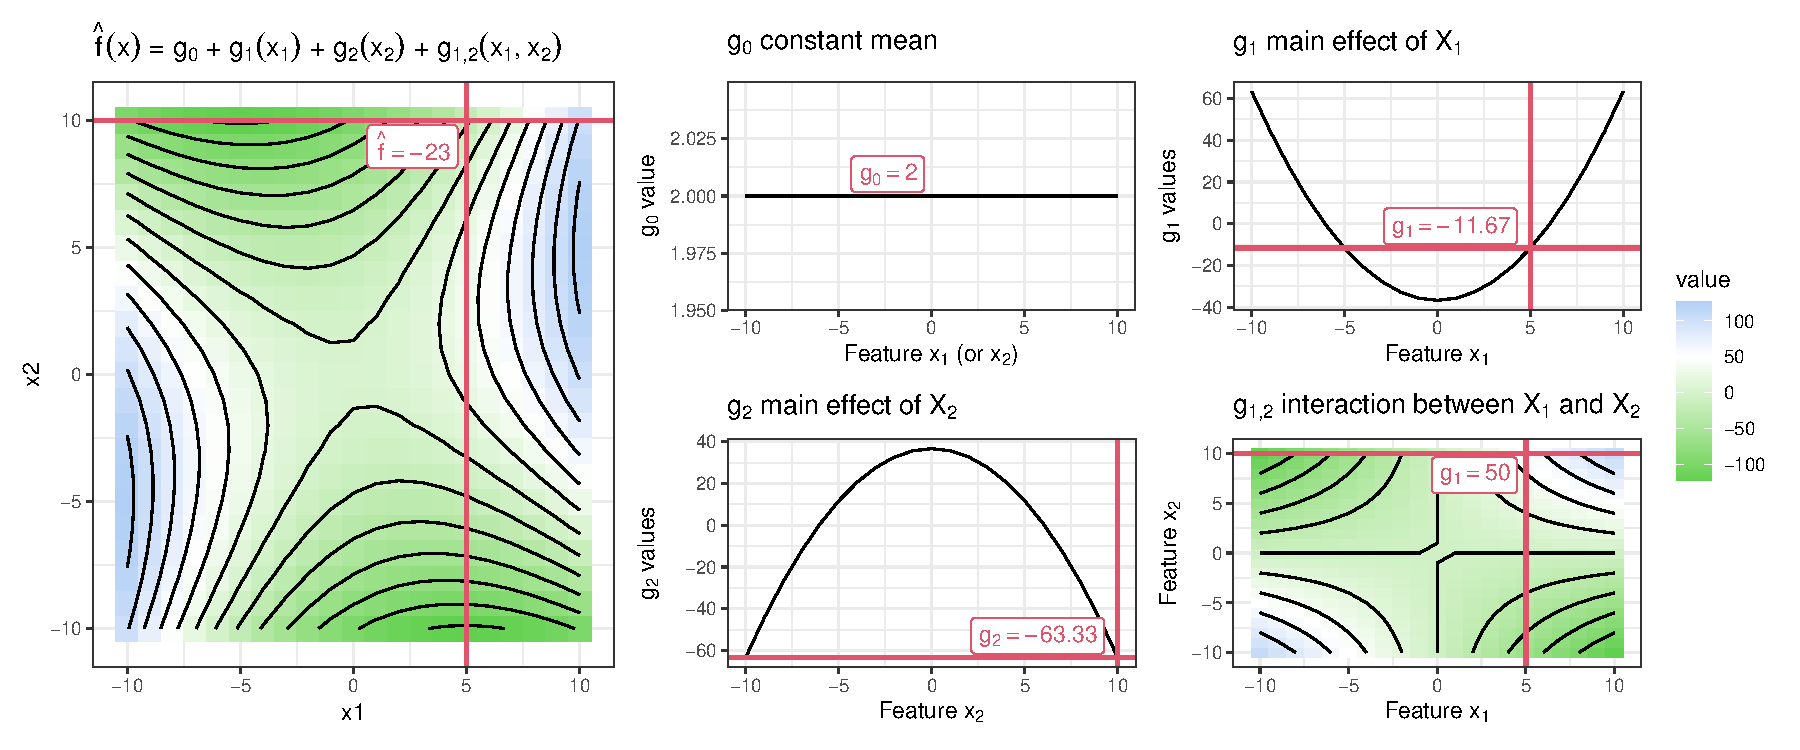
\includegraphics[width = \textwidth]{figure/decomposition}
    % \end{itemize}
    
    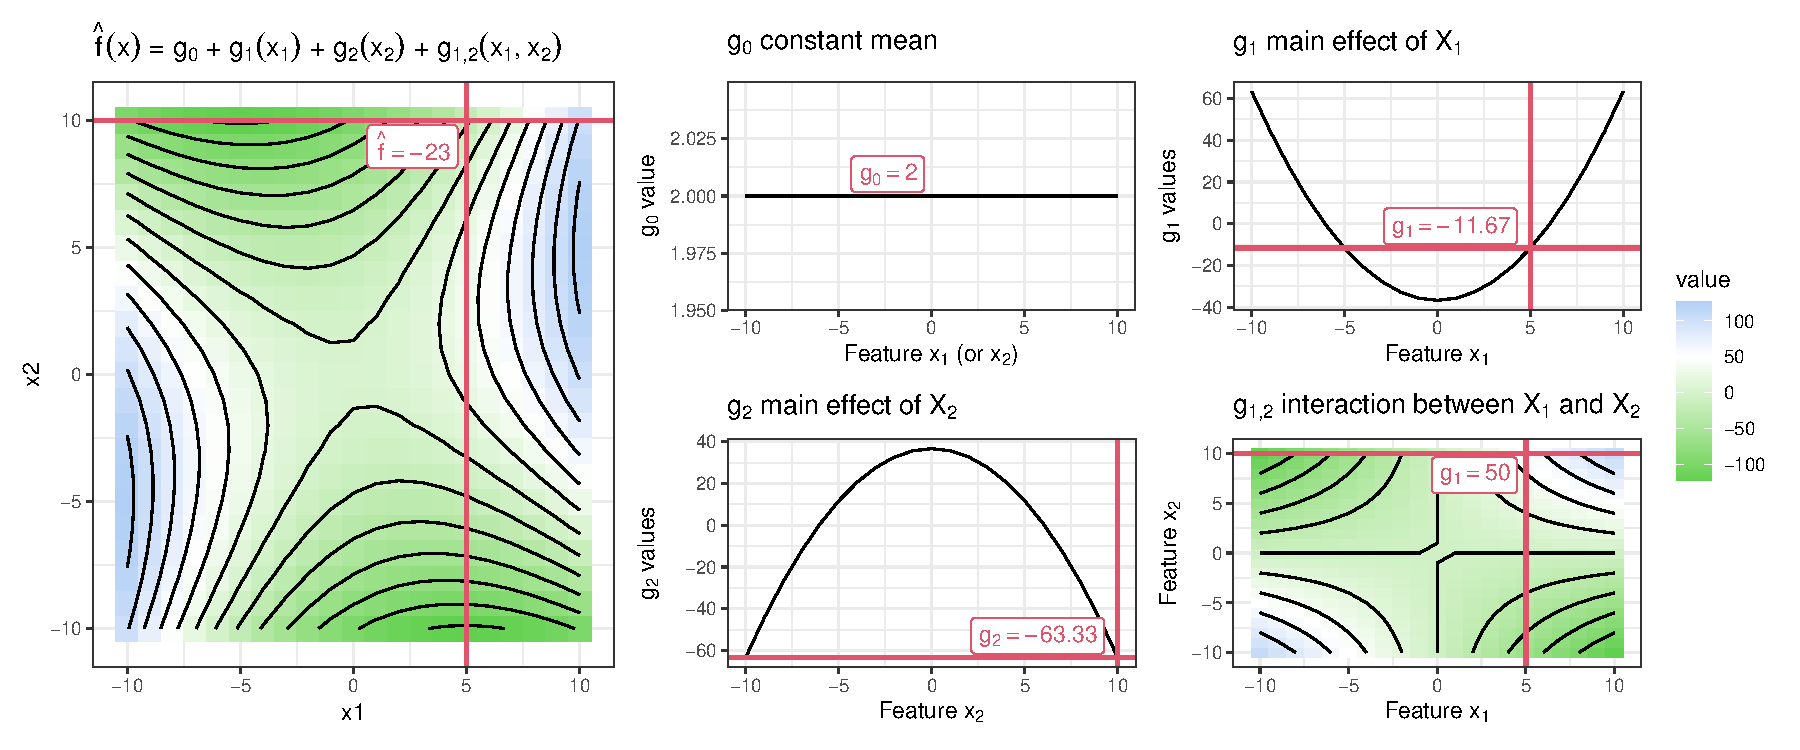
\includegraphics[width = \textwidth]{figure/decomposition}
    
    $\leadsto$ More details on this example later
        
    \end{example}
    
\end{frame}

\begin{frame}{Another example: Additive decomposition}

    \begin{example}

        % Consider the function

        $$
        \fh(x_1, x_2, x_3) = - 2x_1 - 2\sin(x_3) + |x_1|x_2 + 0.5 x_1 x_2 x_3 - \sin(x_2 x_3) + 1
        $$

        % We can again find the additive decomposition by reading from the functional formula, but some terms are empty, because certain types of effects and interactions are not present:
        Again, read additive decomposition from formula:
        \pause
        \begin{equation}\label{eq:func_decomp_second_min_example}
        \begin{aligned}
            & g_\emptyset(x_1, x_2, x_3) = 1 & \text{ constant part, no effects}  \\
            &
            \left.\begin{aligned}
                & g_1(x_1, x_2, x_3) = - 2x_1 \\
                & g_2(x_1, x_2, x_3) = 0 \\
                & g_3(x_1, x_2, x_3) = - 2\sin(x_3)
            \end{aligned}\right\}
                & \text{ main effects, no interactions}  \\
            &
            \left.\begin{aligned}
                & g_{1,2}(x_1, x_2, x_3) = |x_1|x_2 \\
                & g_{1,3}(x_1, x_2, x_3) = 0 \\
                & g_{2,3}(x_1, x_2, x_3) = - \sin(x_2 x_3)
            \end{aligned}\right\}
                & \text{ 2-way interactions (depending on 2 features)}  \\
            & g_{1,2,3}(x_1, x_2, x_3) = 0.5 x_1 x_2 x_3 & \text{ 3-way interactions}  \\
        \end{aligned}
        % \begin{matrix}
        %     g_\emptyset(x_1, x_2) = 4 &  \text{ Parts depending on no features at all (constant)}  \\
        %     g_1(x_1, x_2) = 2x_1 & \text{ Parts depending on a single feature (main effects)} \\
        %     g_1(x_1, x_2) =  0.3 e^{x_2} & \\
        %     g_{1,2}(x_1, x_2) = |x_1|x_2 & \text{ Part depending on both features (interaction)}  \\
        % \end{matrix}
        \end{equation}
        \(\Rightarrow\) 8 components in total, but some empty $\leadsto$ Certain interactions not present
        
    \end{example}
    
\end{frame}

\begin{frame}{General Form of Functional Decomposition
\furtherreading{RABITZ2011}
\furtherreading{CHASTAING2012}
}

\begin{definition}
\textit{Functional decomposition}: Additive decomposition of a function $\fh: \R^p \mapsto \R$ into a sum of components of different dimensions w.r.t. inputs $x_1, \ldots, x_p$: 
\begin{equation*}
\begin{split}
\fh(\xv)
\; = \; \; & \sum_{S \subseteq \{1,\ldots,p\}} g_{S}(\xv_S) \\
\; = \; \; & g_{\open \emptyset \close} +
g_{\open 1 \close}(x_1) + g_{\open 2 \close}(x_2) + \dots + g_{\open p \close}(x_p) + \\
& g_{\open 1, 2 \close}(x_1, x_2) + \dots + g_{\open p-1, p \close}(x_{p-1}, x_p) + \dots + \\
& g_{\open 1, 2, 3 \close}(x_1, x_2, x_3) + \dots +
g_{\open 1, 2, 3, 4 \close}(x_1, x_2, x_3, x_4) + \dots +
g_{\open 1,\ldots,p \close}(x_1, \ldots, x_p)
\end{split}    
\end{equation*}
$\leadsto$ one component for every possible combination $S$ of indices, allowed to formally only depend on these features / be a function of these features
\end{definition}

\textbf{Problems:}
\begin{itemize}
    \item How to find / compute such a decomposition for any black-box models $\fh$?
    \item \dots such that the decomposition is useful / has nice properties (w.r.t. the model / w.r.t. the data)?
\end{itemize}

\end{frame}

\begin{frame}{General Form of Functional Decomposition
%\\
%\furtherreading{SOBOL1993}
% \furtherreading{SOBOL2003}
%\furtherreading{LI2001}
\furtherreading{RABITZ2011}
\furtherreading{CHASTAING2012}
}

%\textbf{High-Dimensional Model Representation (HDMR):} 

\begin{definition}
% For interpretation purposes, one might be interested in decomposing a square-integrable function $\fh: \R^p \mapsto \R$ into sum of components of different dimensions w.r.t. inputs $x_1, \ldots, x_p$: %
\textit{Functional decomposition}: Additive decomposition of a function $\fh: \R^p \mapsto \R$ into a sum of components of different dimensions w.r.t. inputs $x_1, \ldots, x_p$: 
% \begin{equation}
% \begin{split}
% \fh(\xv) = 
% \displaystyle\sum_{S \subseteq \{1,\ldots,p\}} g_{S}(\xv_S) = \; & g_{\open \emptyset \close} + g_{\open 1 \close}(x_1) + g_{\open 2 \close}(x_2) + \dots + g_{\open p \close}(x_p) + \\
% & g_{\open 1, 2 \close}(x_1, x_2) + \dots + g_{\open p-1, p \close}(x_{p-1}, x_p) + \dots + \\
% & g_{\open 1, 2, 3 \close}(x_1, x_2, x_3) + \dots + \dots + g_{\open 1,\ldots,p \close}(x_1, \ldots, x_p)
% \end{split}
% \end{equation}
\begin{equation*}
\begin{split}
\fh(\xv)
\; = \; \; & \sum_{S \subseteq \{1,\ldots,p\}} g_{S}(\xv_S) \\
\; = \; \; & g_{\open \emptyset \close} +
g_{\open 1 \close}(x_1) + g_{\open 2 \close}(x_2) + \dots + g_{\open p \close}(x_p) + \\
& g_{\open 1, 2 \close}(x_1, x_2) + \dots + g_{\open p-1, p \close}(x_{p-1}, x_p) + \dots + \\
& g_{\open 1, 2, 3 \close}(x_1, x_2, x_3) + \dots +
g_{\open 1, 2, 3, 4 \close}(x_1, x_2, x_3, x_4) + \dots +
g_{\open 1,\ldots,p \close}(x_1, \ldots, x_p)
\end{split}    
\end{equation*}
$\leadsto$ one component for every possible combination $S$ of indices
\end{definition}
Sort terms according to degree of interaction:
\begin{itemize}
\item $g_{\open \emptyset \close} \hat = $ Constant mean (intercept) %$\mathbb{E}_X (\fh(\xv)) $
\item $g_{\open j \close} \hat = $ first-order or main effect of $j$-th feature alone on $\fh(\xv)$
\item $g_{\open j, k \close} \hat = $ second-order interaction effect of features $j$ and $k$ w.r.t. $\fh(\xv)$%, etc.
\item $g_{S}(\xv_S) \hat = $ $|S|$-order effect, depends \textbf{only} on features in $S$ %$x_j$ for all $j \in S$
\end{itemize}
\lz
\end{frame}

% TO DO: Put an example from a real-world dataset here for illustration purposes

\begin{frame}{Properties of the definition}
\begin{itemize}
    \item \textbf{Interpretability}: Extremely powerful decomposition, reveals complete interaction structure
    \pause
    \item Compare to GAM: Same decomposition, but without interactions \\
    $\implies$ Any GAM already comes with its decomposition
    $$
    \fh (\xv) = g_\emptyset + g_1(x_1) + g_2(x_2) + \ldots + g_p(x_p)
    $$
    \item Same for LMs: Decomposition explicitly modeled
    \pause
    \item Easy decomp. also for decision trees and tree ensembles (see below)
    \pause
    \item \textbf{Problem 1:} Calculating decomposition extremely difficult, often infeasible
    \begin{itemize}
        \item For \(p\) features: Decomposition with \(2^p\) terms \(\rightarrow\) too many different terms, difficult to interpret
    \end{itemize}
    \pause
    \item \textbf{Problem 2:} Definition not complete: Decomposition not unique, many trivial decompositions not useful
    \begin{itemize}
        \item[$\rightarrow$] More requirements or constraints needed to ensure decomposition is meaningful
        \item Even worse once features are dependent or correlated (see later)
    \end{itemize}
    % This 
    % Compare to GAM: The same decomposition is used, but in case of GAM, no interactions at all are considered, only main effects. I.p. any GAM already comes with its decomposition! \\
    % Same for linear models / linear regression and GLMs: The decomposition is explicitly modeled and directly follows from the model structure.

    % Somewhat similar for decision trees and tree ensembles (see below)
    % Super nice and extremely powerful decomposition! "Holy Gral of interpreting complex models"\\
    % BUT 2 Problems:
    % \begin{itemize}
    %     \item Definition not complete, such decomposition is not unique, and many trivial decompositions are not useful at all (see next slide) \\
    %         This problem get's much worse, whenever features are not independent \\
    %     \textbf{N.B.:} %Further constraints are required to obtain an unique and optimal solution for the components
    %     A unique solution for the components only exists under certain assumptions $\leadsto$ constraints, see later
        %and constraints
        %independent inputs and a \textit{vanishing condition}
        %$$\mathbb{E}_{X_j} (g_{S}(\xv_S)) = \int g_{S}(\xv_S) d \mathbb{P}(x_j) = 0, \forall j \in S, \forall S \subseteq \{1, \ldots, p\}$$
        %Without further constraints on components, there is no unique solution.
        %\end{itemize}
    %     \item Calculating such a decomposition is super, super hard in practice \\
    %         See for example: For \(p\) features, the decomposition has \(2^p\) terms \(\Rightarrow\) not very meaningful to interpret so many different terms \\
    % \end{itemize}
\end{itemize}
\end{frame}

\begin{frame}{Problem 2: Definition not enough}

    \begin{example}
        Again consider
        $$
        \fh(x_1, x_2, x_3) = - 2x_1 - 2\sin(x_3) + |x_1|x_2 + 0.5 x_1 x_2 x_3 - \sin(x_2 x_3) + 1
        $$
        \pause
        Two possible decompositions (valid according to definition):
        $$
            g_{1, \dots, p}(x_1, \dots, x_p) := \fh(\xv) \text{ and for all other terms } g_S(\xv_S) := 0 ,
        $$
        or:
        \begin{align*}
            g_\emptyset & = 1 \,;\quad
            g_1(x_1) = x_1 \,;\;
            g_2(x_2) = 2x_2 \,;\;
            g_3(x_3) = 3x_3 \,;\quad \\
            g_{1,2}(x_1, x_2) & = \frac{1}{2} x_1 x_2 \,;\;
            g_{1,3}(x_1, x_3) = \frac{1}{3} x_1 x_3 \,;\;
            g_{2,3}(x_2, x_3) = \frac{2}{3} x_2 x_3 \,;\; \\
            \text{ and} \quad
            & g_{1,2,3}(x_1, x_2, x_3) = \fh(x_1, x_2, x_3) - \sum_{S \subsetneqq \{1,2,3\}} g_S(\xv_S)
        \end{align*}
    \end{example}
    % Use $g_{1, \dots, p}(x_1, \dots, x_p) := \fh(\xv)$ and $g_S(\xv_S) := 0$ for all other terms
    \pause
    \(\implies\) Definition of decomposition not unique \\
    
\end{frame}

\begin{frame}{Example: Decision Trees}

\only<1,2>{
Define \textit{interaction type $t$} of a node: subset of features used to build this node.

\textbf{Example:}

\begin{center}
    \begin{tikzpicture}[
    node/.style = {scale=1},
    scale = 1
    ]
        
        \node[node] at (0,2)(root){\(\R^d\)};
        
        \node[node] at (3,.5)(right_child){\(x_2 > 0\)};
        \node[node] at (4,-1)(rightright_grandchild){$x_3 > 1$};
        \node[node] at (2,-1)(rightleft_grandchild){\(x_3 \leq 1\)};
        
        \node[node] at (-3,.5)(left_child){\(x_2 \leq 0\)};
        \node[node] at (-4,-1)(leftleft_grandchild){$x_4 \leq -1$};
        \node[node] at (-1,-1)(leftright_grandchild){\(x_4 > -1\)};
        
        \node[node] at (-2,-2.5)(low_child_1){$x_1 \leq -0.5$};
        \node[node] at (-0,-2.5)(low_child_2){$x_1 > -0.5$};

        \draw[->, shorten >= 1pt, shorten <= 1pt] (root) -- (left_child);
        \draw[->, shorten >= 1pt, shorten <= 1pt] (root) -- (right_child);
        \draw[->, shorten >= 1pt, shorten <= 1pt] (left_child) -- (leftleft_grandchild);
        \draw[->, shorten >= 1pt, shorten <= 1pt] (left_child) -- (leftright_grandchild);
        \draw[->, shorten >= 1pt, shorten <= 1pt] (right_child) -- (rightright_grandchild);
        \draw[->, shorten >= 1pt, shorten <= 1pt] (right_child) -- (rightleft_grandchild);
        
        \draw[->, shorten >= 1pt, shorten <= 1pt] (leftright_grandchild) -- (low_child_1);
        \draw[->, shorten >= 1pt, shorten <= 1pt] (leftright_grandchild) -- (low_child_2);

        \only<2>{
        \node[node, color=red] at (0,1.5)(root_type){$t=\{\}$};
        
        \node[node, color=red] at (3,0)(right_child_type){$t=\{2\}$};
        \node[node, color=red] at (4,-1.5)(rightright_grandchild_type){$t=\{2,3\}$};
        \node[node, color=red] at (2,-1.5)(rightleft_grandchild_type){$t=\{2,3\}$};
        
        \node[node, color=red] at (-3,0)(left_child_type){$t=\{2\}$};
        \node[node, color=red] at (-4,-1.5)(leftleft_grandchild_type){$t=\{2,4\}$};
        \node[node, color=red] at (-1,-1.5)(leftright_grandchild_type){$t=\{2,4\}$};
        
        \node[node, color=red] at (-2,-3)(low_child_1_type){$t=\{1,2,4\}$};
        \node[node, color=red] at (0,-3)(low_child_2_type){$t=\{1,2,4\}$};
        
        }

    \end{tikzpicture}
\end{center}
}

\only<2>{
$\Rightarrow$ Degree of interaction in each node is \(|t|\).
}
    
\end{frame}

\begin{frame}{Decomposition for Decision Trees}
    
% [show that one decision tree directly comes with its functional decomposition using indicator functions]\\

Here: Decomposition via indicator functions
$$
\fh(\xv) = g_\emptyset + g_{2,4}(x_2, x_4) + g_{2,3}(x_2, x_3) + g_{1, 2, 4}(x_1, x_2, x_4)
$$
$\implies$ Decomposition has no main effect, but model certainly contains an effect of e.g. $x_2$

$\implies$ Lower-order effects ``hidden'' inside higher-order terms

$\leadsto$ reading from decision tree not enough, ``bad decomposition''

% \textbf{Problem again: uniqueness} If only reading from decision tree using indicator functions, lower-order effects may be hidden inside higher-order terms? \\

% Above example: Decomposition no main effect, but model certainly contains main effect of e.g. $x_2$.\\

\pause
\medskip
\textbf{Note:} \furtherreading{YANG2024} propose a (quite complicated) solution for this case
% \(\Rightarrow\) Too complicated? Rather explain this in constraint-chapter or in other methods-chapter?

\end{frame}



\begin{frame}{Example: EBM}

    \begin{itemize}
        \item See before: \textbf{GAMs} have functional decomposition by definition
        \item \textbf{EBMs:} Sum of the final one- and two-dimensional components
        % \item \textbf{Similar: EBMs} Use the final one- and two-dimensional components % visualized in the end
        {
        \centering
        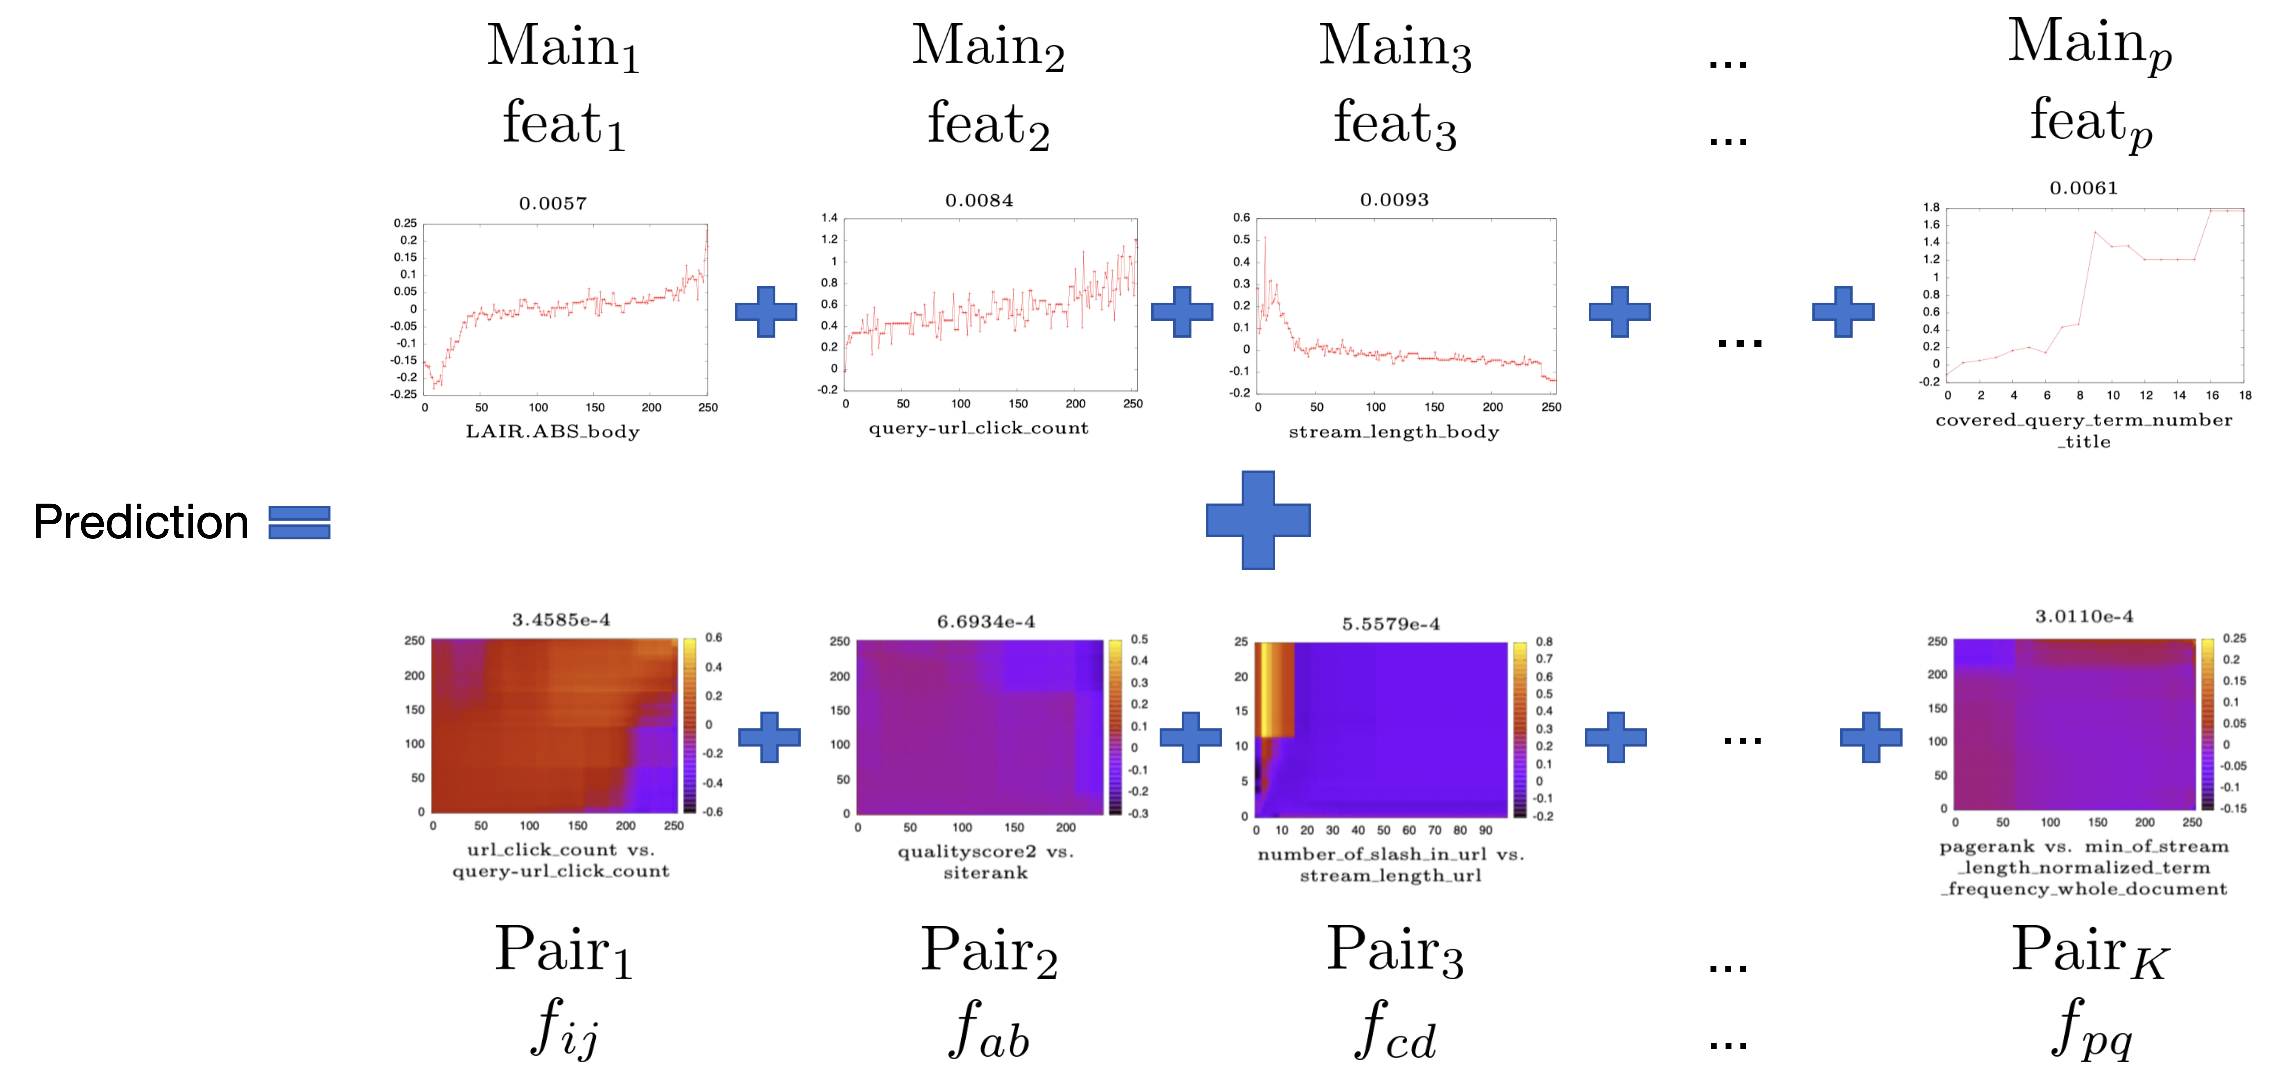
\includegraphics[width=\linewidth]{figure/final_ebm.png}
        }
        \only<2>{
        \item In general: Model with functional decomposition up to max. order 2 is always ``inherently interpretable''
        \item \textbf{Reason:} Visualization of all components
        } 
    \end{itemize}
    
\end{frame}

% \begin{frame}{High-dimensional modl representation (HDMR)}
%     [explain link to HDMR?? Or at end of chapter ?]

%     same for Sobol-Hoeffding decomposition
% \end{frame}

\endlecture
\end{document}
